\section{Introduction}\label{sec:intro}

Text-to-motion generation has made striking progress, but almost all of it on one body. The standard
pipeline---a diffusion model, a motion tokeniser or a latent generator trained on
HumanML3D~\citep{guo2022generating}---assumes a fixed kinematic tree, typically the 22-joint SMPL
skeleton, and bakes it into every layer: the input projection is sized for that joint count and any
codebook is learned for one morphology. The result is a family of models that animate a human well and
cannot animate anything else. The applications that most need generative motion---games, film
previsualisation, virtual production---are populated by characters that are not human, and a studio does
not have one skeleton but hundreds, each authored by a rigger and each with its own joint count, naming
scheme and helper bones.

\begin{figure}[t]
\centering
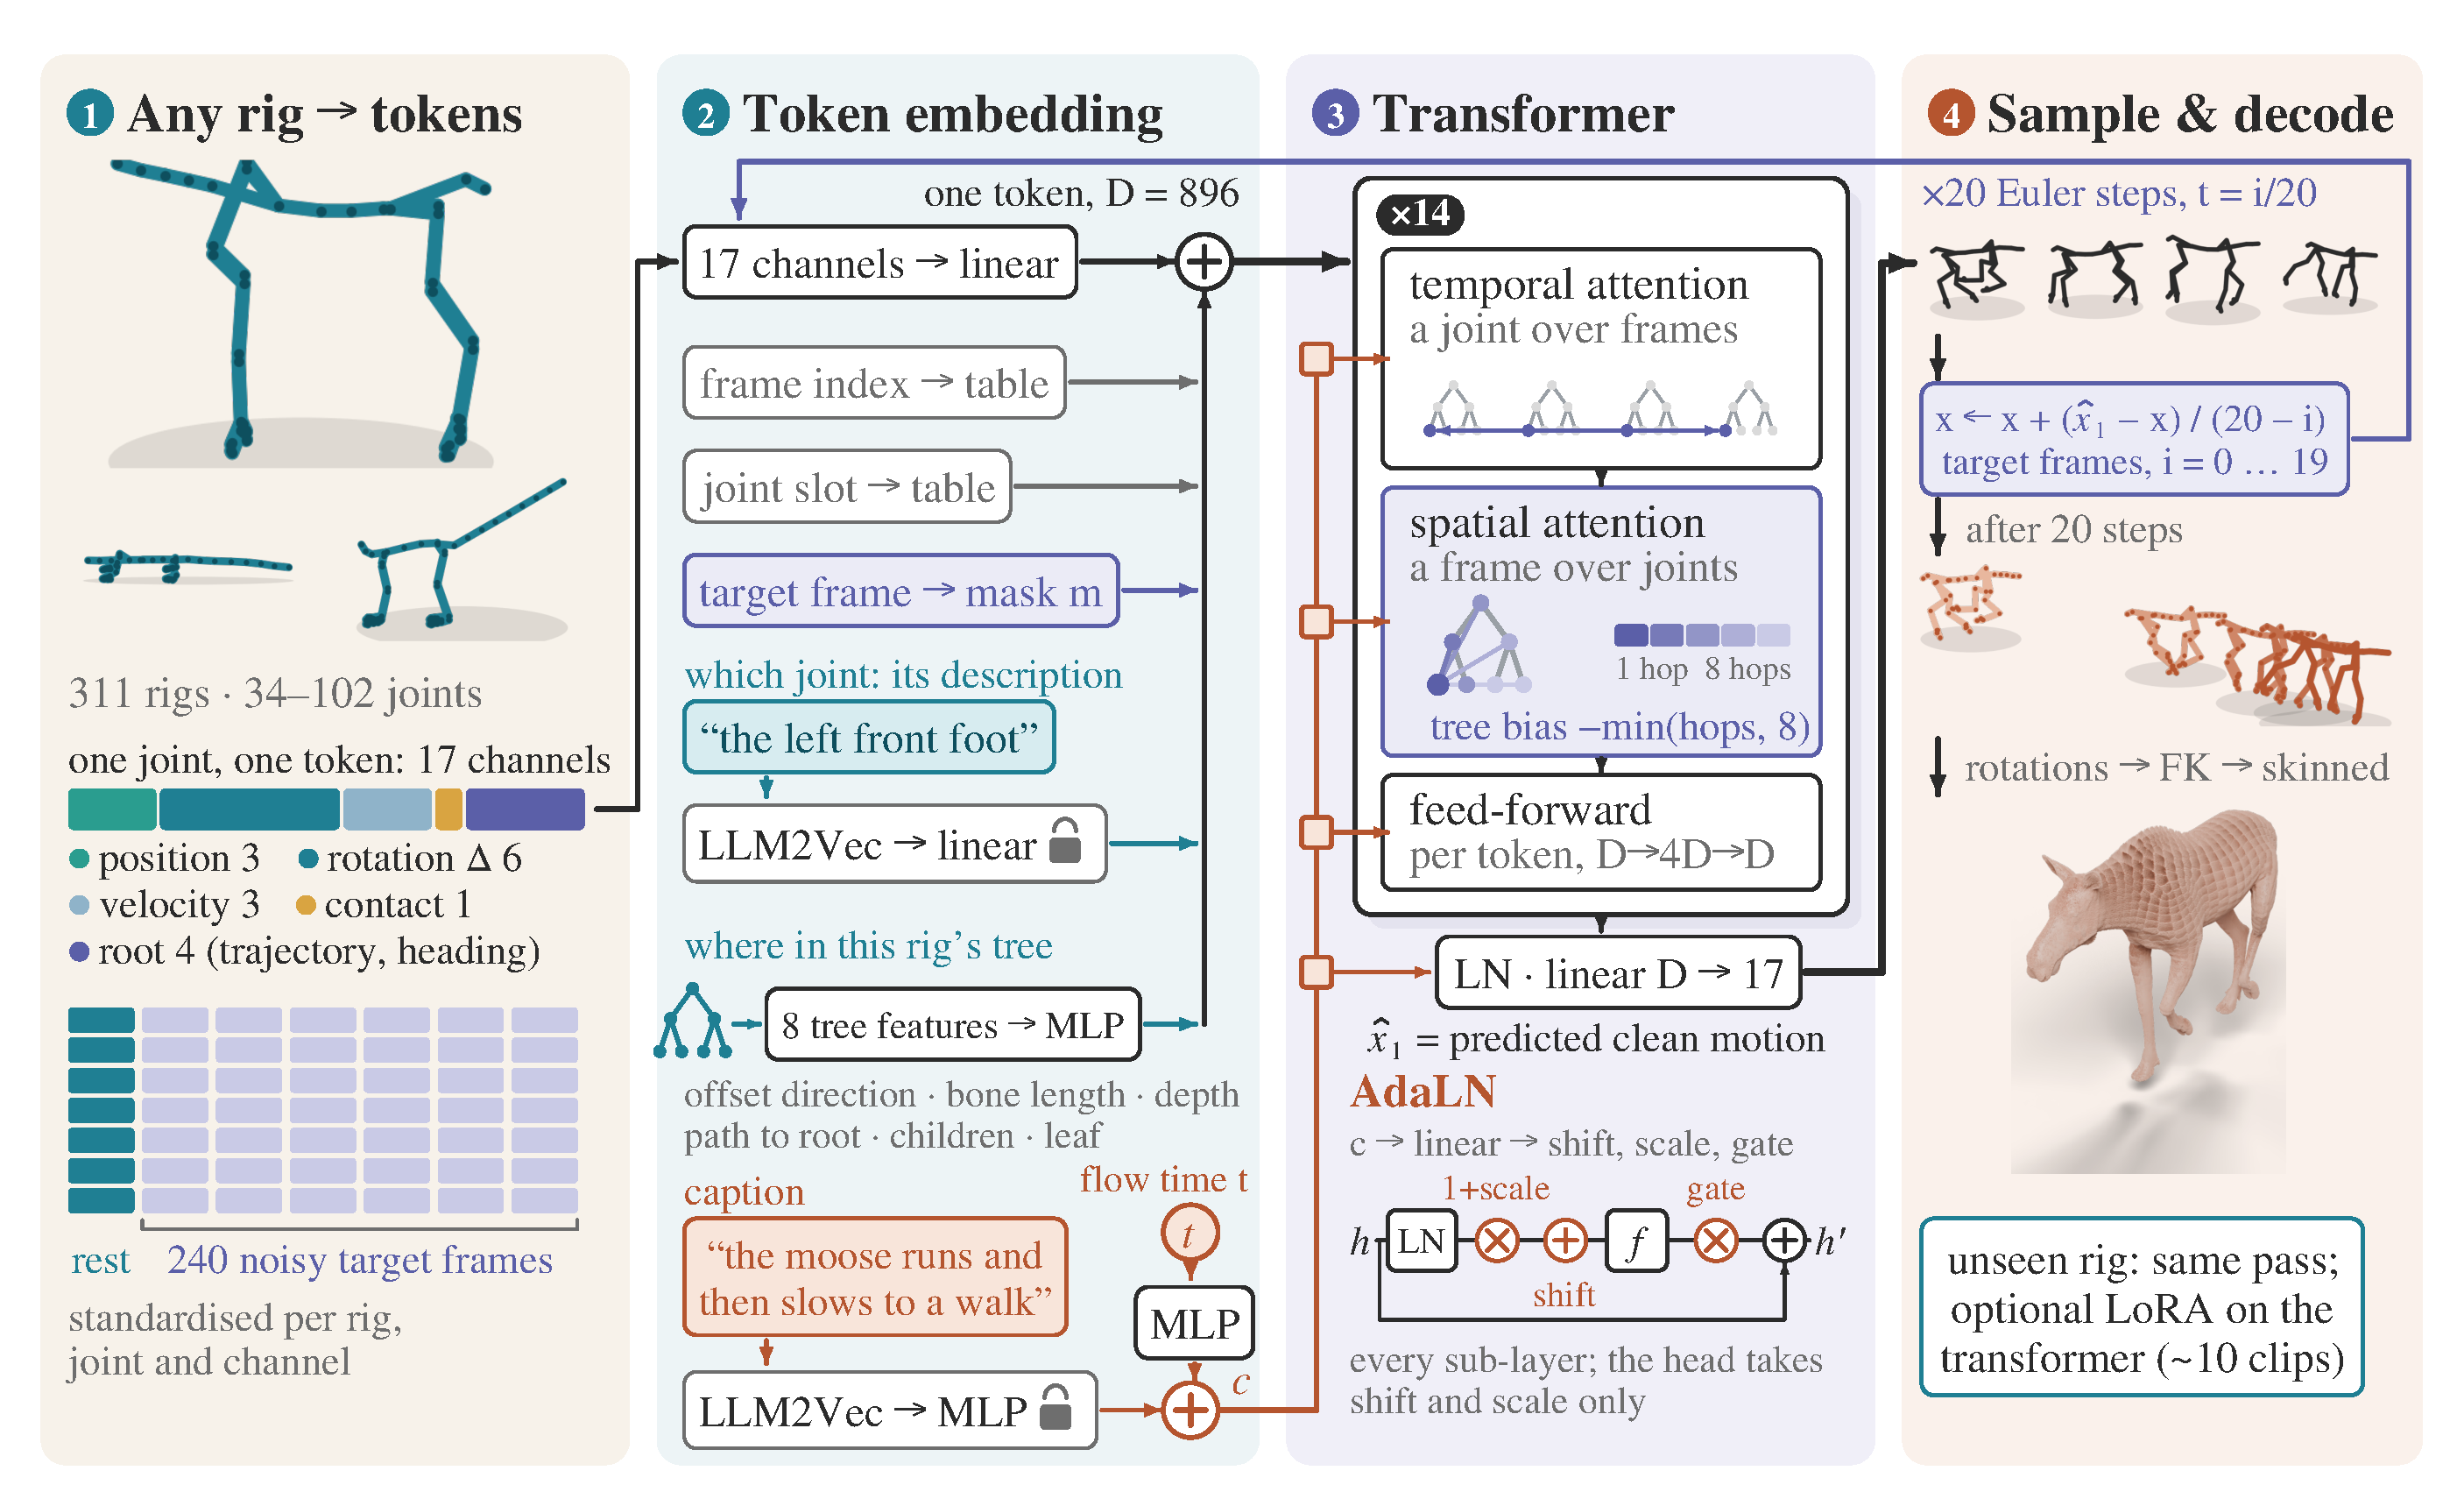
\includegraphics[width=\linewidth]{figures/fig1_align/figure1.pdf}
\caption{\method{} overview. A rig enters as data: one token per joint and frame with 17 standardised
channels, and the sequence is the rig's clean rest pose followed by the noise-mixed target frames. The
skeleton enters through the token sum (panel~2) and a tree-distance bias on spatial attention; the caption
and the flow time modulate every block through AdaLN. The head predicts the clean motion, the Euler steps
update the target frames only, and the rotations are played on the rig. An unseen rig takes the same pass.
All skeleton drawings are the model's own output on a moose run-to-walk clip.}\label{fig:teaser}
\end{figure}

\paragraph{Why one model for many skeletons is hard.} Four things stand in the way. There is no common
tensor: rigs differ in joint count, joint order, naming and scale, so cross-skeleton work has either
\emph{retargeted} onto a canonical skeleton~\citep{villegas2018nkn,aberman2020skeleton,lee2023same}, which
degrades as morphology diverges, or fixed a template body plan, which excludes every other body. The network
has to be told what each joint of an unfamiliar tree is and how the joints relate, without a parameter per
skeleton. A loss summed over a batch of rigs with 34 to 102 joints lets the largest bodies dominate, and
training such a model at 0.3B parameters is unstable without care. And a rig outside the training library has
to be served with no clips, or a handful, because a model per character multiplies data and compute by the
size of the cast. Generation across skeletons has been shown without text by AnyTop~\citep{gat2025anytop} on
the Truebones zoo, and with text by OmniZoo~\citep{chen2025omnizoo} on 140 species and by
G-MDM~\citep{lee2025dragon} on Truebones with joint rotations but no root translation.

\paragraph{Our position.} A generative model should treat the skeleton as \emph{input}, not as
architecture: told the kinematic tree, the rest pose and what each joint is, the network needs no
per-skeleton parameter, and adding a character becomes a data question. We study text-conditioned
generation of joint rotations and root trajectories across \num{311} production rigs at 0.3B parameters, on a
corpus that is a faithful sample of studio reality: \num{311} animal rigs with \num{34} to \num{102}
deformation joints (median 64), \num{108} distinct kinematic trees and \num{77{,}894} captioned clips
(\num{6.2}M frames).\footnote{The clips and their captions follow the AniMo4D annotation set of
\citet{wang2025animo}; the rigs are re-exported with deformation bones only, the joint descriptions are ours,
and the conversion to \rep{} is new (App.~\ref{app:rep}). The Truebones zoo, a publicly distributed set of 66
animal rigs, is kept entirely outside training.} The output is what a rig plays, per-joint rotations and a
world-space root trajectory, with no inverse-kinematics fit.

\paragraph{Contributions.}
\begin{enumerate}[leftmargin=*,itemsep=1pt,topsep=2pt]
\item \textbf{One text-to-motion system for hundreds of production skeletons, at 0.3B parameters}
  (\S\ref{sec:exp:main}). A single network trained on \num{311} rigs generates text-conditioned motion for
  every one of them and returns what the rig plays---rotations and a world-space root trajectory, no
  inverse-kinematics fit. The recipe trains a \num{303}M model stably, and retrieval and FID improve
  monotonically from \num{36}M to \num{303}M parameters.
\item \textbf{\rep{}, a motion representation designed so that any rigged animation becomes training data}
  (\S\ref{sec:method:rep}). A clip is converted from its kinematic tree, rest pose and motion alone---no
  template, retargeting, tokeniser or inverse kinematics---and every (rig, joint, channel) cell is
  standardised by its own statistics, which is what lets rigs of very different proportions share one
  network: 1.7--2.0 points of R@1 over a per-rig scale.
\item \textbf{Skeleton awareness inside the model: a rest-pose prompt and graph-biased attention}
  (\S\ref{sec:method:model}). The rig's clean rest pose leads the token sequence, and a tree-distance bias
  with learned ancestor tables lets spatial attention tell parent from child and one limb from another.
  Nothing in the network is indexed by rig, so a new rig is a new input; the flat padded-joint construction
  that fixed-skeleton generators are usually brought to variable skeletons with trails this design by
  0.19--0.20 of R@1.
\item \textbf{High fidelity in the library and zero- and few-shot generalisation outside it}
  (\S\ref{sec:exp:extend}). \method{} reaches R@1 \num{0.867} against \num{0.904} for the real clips and
  FID \num{0.005}. A rig the model has never seen is served by the same forward pass, and a low-rank adapter
  on roughly ten clips brings its rotation and position channels into agreement on bodies far from the
  training distribution (a winged dragon: from \num{4.46} to \num{0.30} bone lengths).
\end{enumerate}
